\section{Extended design figures and subsystem evidence}\label{app:des-visual-tests}
\subsection{Recorded capture and seam checks}
\begin{table}[H]\centering\small
\begin{tabular}{lrrrrr}\hline
Page & Label lines & Reduced & Gradient & $+3^\circ$ & $90^\circ$ \\\hline
Owen & 20 & 19 & 20 & 11 & 19 \\
Dylan & 24 & 24 & 24 & 25 & 24 \\
Yeukita & 26 & 26 & 26 & 26 & 26 \\
\hline\end{tabular}
\caption{Exploratory crop counts after extra input reduction and digital perturbation. Equal counts do not establish correct ink ownership.}
\label{tab:des-resample-cases}
\end{table}
\begin{table}[H]\centering\small
\begin{tabular}{|c|c|r|r|r|}
\hline Midpoint weight&Step penalty&Ink intersections&Row movement&Mean offset / px\\\hline
0.000&0.020&2&35&4.0553\\\hline
0.006&0.020&2&38&0.5517\\\hline
0.012&0.020&2&42&0.3625\\\hline
0.024&0.020&2&44&0.3261\\\hline
0.048&0.020&2&47&0.2622\\\hline
0.012&0.000&2&48&0.2622\\\hline
0.012&0.010&2&44&0.3261\\\hline
0.012&0.040&2&38&0.5517\\\hline
\end{tabular}
\caption{New coefficient-sensitivity check across six fixed real-page gaps; the implemented setting is 0.012/0.020.}
\label{tab:app-seam-sweep}
\end{table}
\label{app:des-seam-sweep}
\subsection{Numerical verification records}\label{sec:des-netverify}
Figure~\ref{fig:vt-grad} compares analytic gradients with finite differences.
\begin{figure}[H]\centering
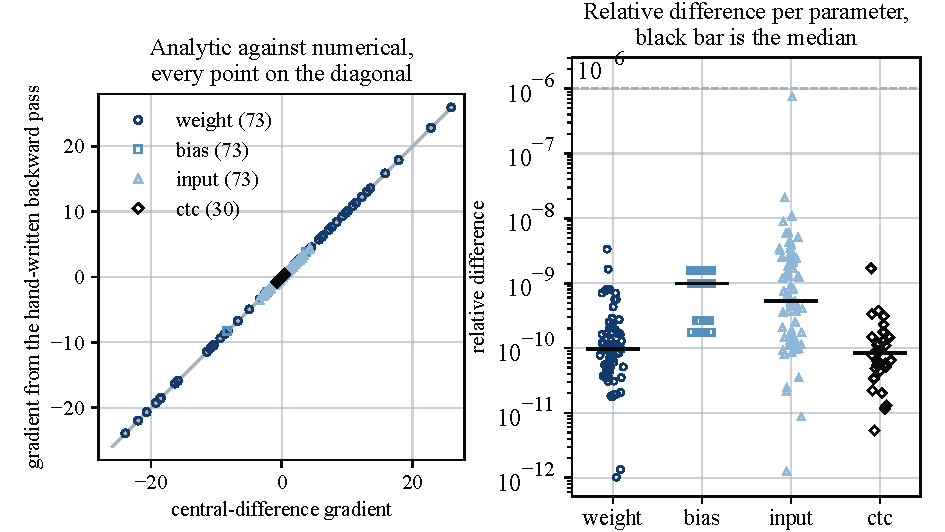
\includegraphics[width=\linewidth]{Figures/VisualTests/T38_gradient_check.pdf}
\caption{Analytic and finite-difference gradients.}
\label{fig:vt-grad}
\end{figure}
Figure~\ref{fig:vt-width} extends the normalisation-width sweep.
\begin{figure}[H]\centering
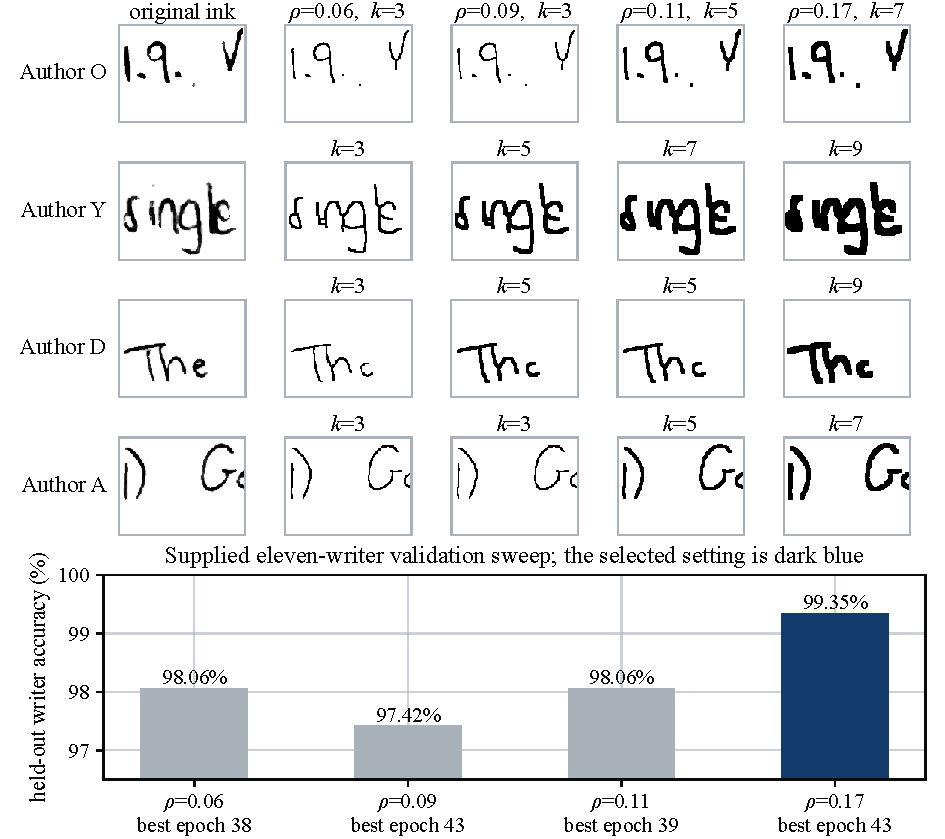
\includegraphics[width=\linewidth]{Figures/VisualTests/T40_stroke_width_sweep.pdf}
\caption{Stroke-width kernels and validation sweep.}
\label{fig:vt-width}
\end{figure}
Figure~\ref{fig:vt-coordinates} shows the recorded glyph coordinate frames.
\begin{figure}[H]\centering
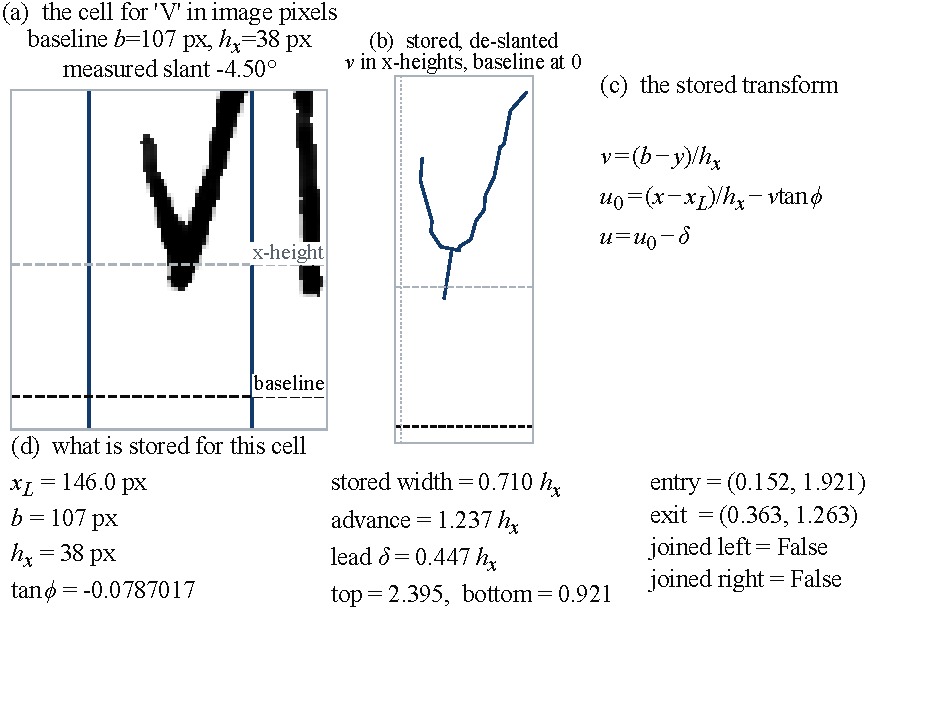
\includegraphics[width=\linewidth]{Figures/VisualTests/T43_glyph_coordinates.pdf}
\caption{Image and stored glyph coordinate frames.}
\label{fig:vt-coordinates}
\end{figure}
\subsection{Extended figures from the Design section}\label{app:extended-design-figures}
Figure~\ref{fig:vt-seamfield} extends the seam examples retained in Design.
\begin{figure}[H]\centering
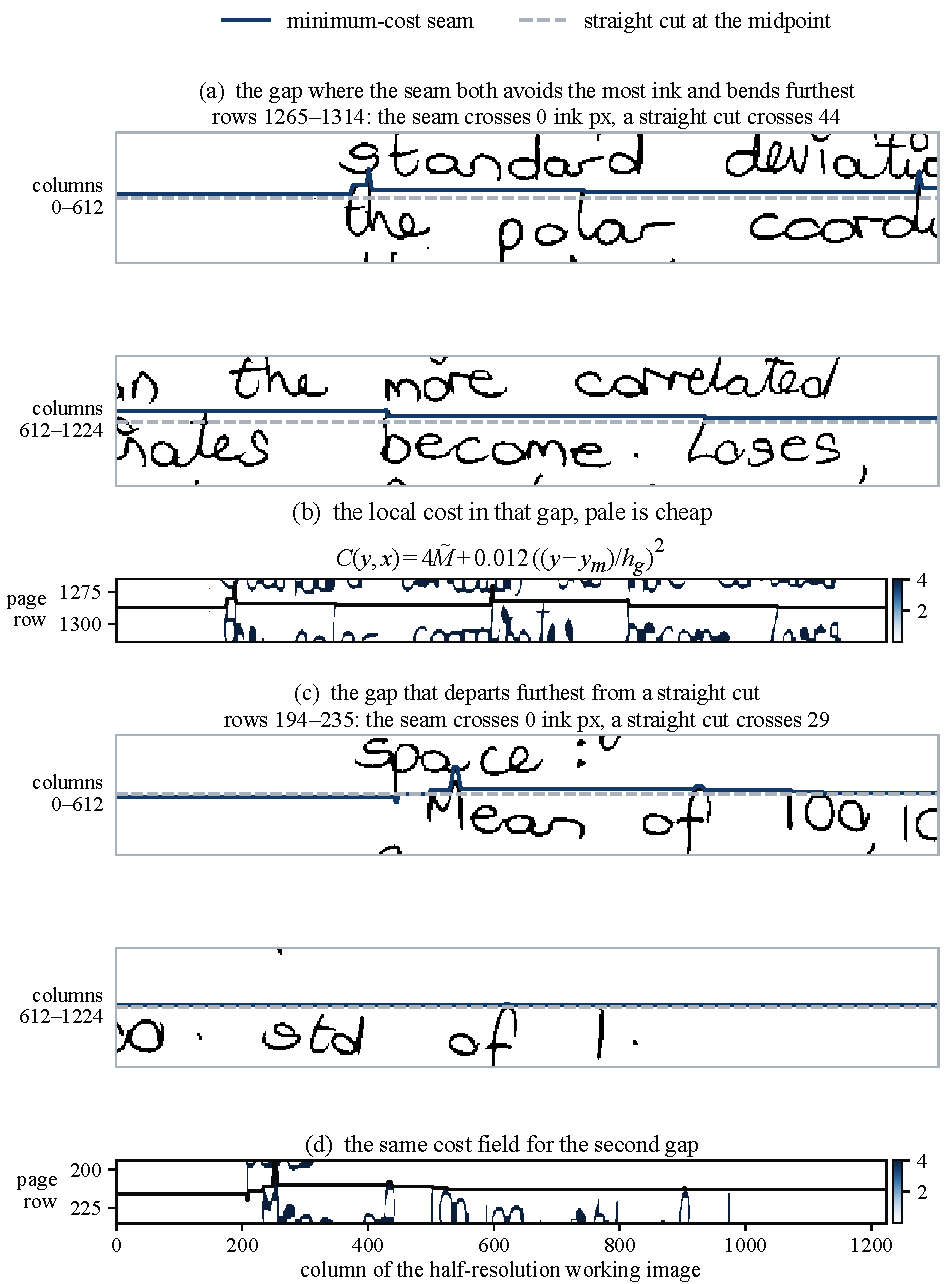
\includegraphics[width=\linewidth]{Figures/VisualTests/T25_seam_cost_field.pdf}
\caption{Complete seam and cost-field examples.}
\label{fig:vt-seamfield}
\end{figure}
Figure~\ref{fig:vt-featurestack} shows the complete feature sequence.
\begin{figure}[H]\centering
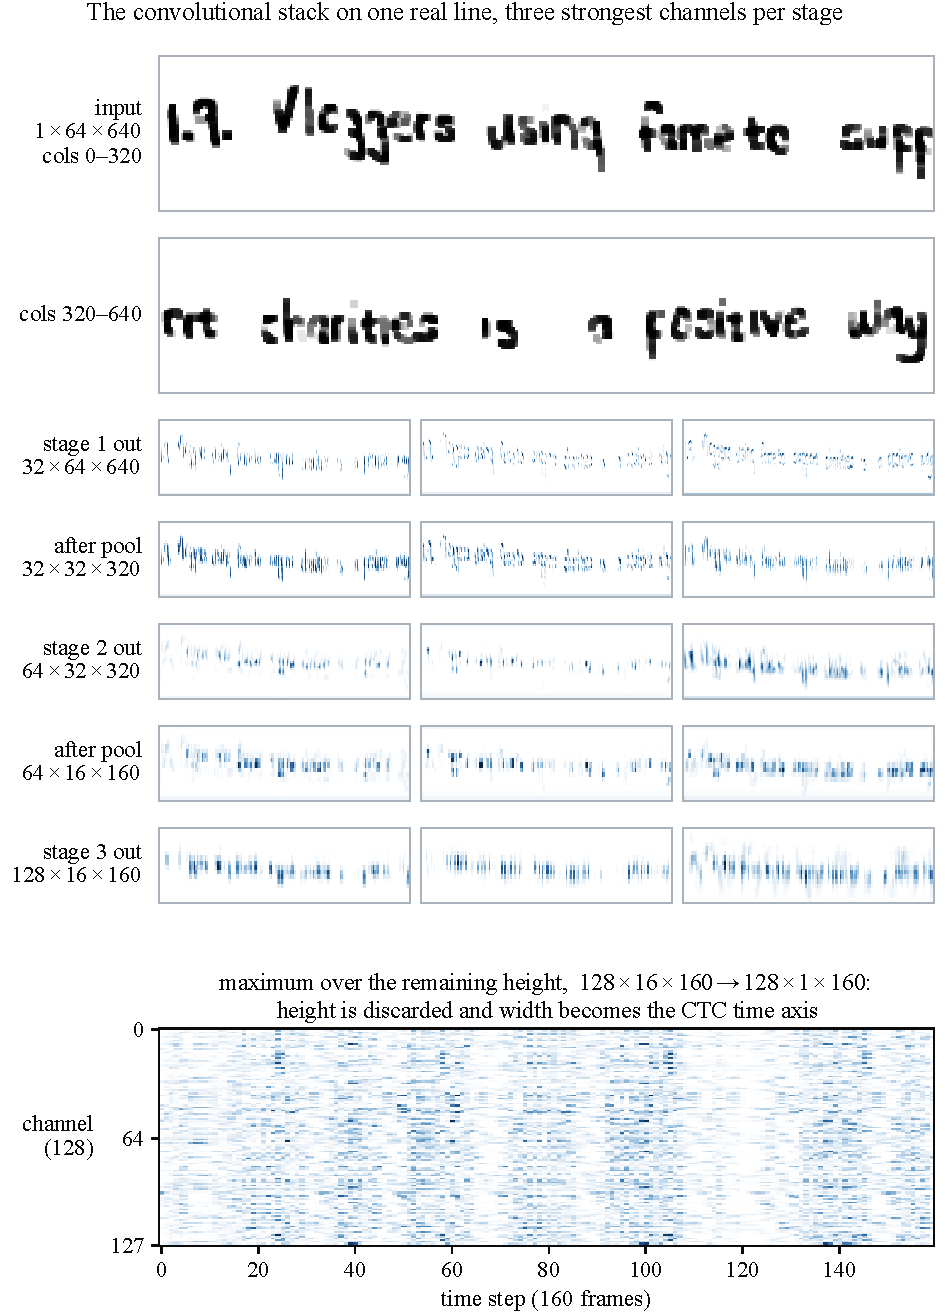
\includegraphics[width=\linewidth]{Figures/VisualTests/T32_feature_stack.pdf}
\caption{Complete convolutional feature sequence.}
\label{fig:vt-featurestack}
\end{figure}
\FloatBarrier
